\documentclass{beamer}
\usetheme[numbering=progressbar]{focus}
\definecolor{main}{RGB}{47, 161, 219}
\definecolor{textcolor}{RGB}{128, 128, 128}
\definecolor{background}{RGB}{240, 247, 255}


\usepackage[utf8x]{inputenc}
\usepackage{listings}
\usepackage{soul}
\usepackage{siunitx}
\usepackage{booktabs}
%\lstset{ 
%  backgroundcolor=\color{white},   % choose the background color; you must add \usepackage{color} or \usepackage{xcolor}
%  basicstyle=\footnotesize,        % the size of the fonts that are used for the code
%  breakatwhitespace=false
%}

\usepackage{tikz}
\usetikzlibrary{shapes,snakes,automata,positioning}

\usepackage{xcolor}
\usepackage{colortbl}
\definecolor{mygreen}{rgb}{0,0.6,0}
\definecolor{mygreen2}{rgb}{0,0.56,0.16}
\definecolor{myred}{rgb}{0.6,0.066,0.066}
\definecolor{redCIRCL}{RGB}{213,43,30}
\definecolor{mygray}{rgb}{0.5,0.5,0.5}
\definecolor{mymauve}{rgb}{0.58,0,0.82}
\definecolor{mygray}{gray}{0.9}
\definecolor{mywhite}{rgb}{1,1,1}
\definecolor{myblack}{rgb}{0,0,0}
\definecolor{mybeige}{HTML}{eeeeee}
%\usepackage{tcolorbox}
\usepackage[listings]{tcolorbox}
\tcbuselibrary{listings}

\lstdefinestyle{code}{ %
  backgroundcolor=\color{mybeige},   % choose the background color; you must add \usepackage{color} or \usepackage{xcolor}; should come as last argument
  basicstyle=\footnotesize\ttfamily,        % the size of the fonts that are used for the code
  breakatwhitespace=false,         % sets if automatic breaks should only happen at whitespace
  breaklines=true,                 % sets automatic line breaking
  captionpos=b,                    % sets the caption-position to bottom
  commentstyle=\color{mygreen},    % comment style
  deletekeywords={...},            % if you want to delete keywords from the given language
  escapeinside={\%*}{*)},          % if you want to add LaTeX within your code
  extendedchars=true,              % lets you use non-ASCII characters; for 8-bits encodings only, does not work with UTF-8
  frame=single,	                   % adds a frame around the code
  keepspaces=true,                 % keeps spaces in text, useful for keeping indentation of code (possibly needs columns=flexible)
  keywordstyle=\color{blue},       % keyword style
  language=Python,                 % the language of the code
  morekeywords={*,...},           % if you want to add more keywords to the set
  numbers=left,                    % where to put the line-numbers; possible values are (none, left, right)
  numbersep=5pt,                   % how far the line-numbers are from the code
  numberstyle=\tiny\color{myblack}, % the style that is used for the line-numbers
  rulecolor=\color{black},         % if not set, the frame-color may be changed on line-breaks within not-black text (e.g. comments (green here))
  showspaces=false,                % show spaces everywhere adding particular underscores; it overrides 'showstringspaces'
  showstringspaces=false,          % underline spaces within strings only
  showtabs=false,                  % show tabs within strings adding particular underscores
  stepnumber=1,                    % the step between two line-numbers. If it's 1, each line will be numbered
  stringstyle=\color{mymauve},     % string literal style
  tabsize=2,	                   % sets default tabsize to 2 spaces
  title=\lstname                   % show the filename of files included with \lstinputlisting; also try caption instead of title
}
\lstdefinestyle{bash}{ %
  backgroundcolor=\color{black!85},   % choose the background color; you must add \usepackage{color} or \usepackage{xcolor}; should come as last argument
  basicstyle=\footnotesize\color{mywhite},        % the size of the fonts that are used for the code
  breakatwhitespace=false,         % sets if automatic breaks should only happen at whitespace
  breaklines=true,                 % sets automatic line breaking
  captionpos=b,                    % sets the caption-position to bottom
  commentstyle=\color{mygreen},    % comment style
  deletekeywords={...},            % if you want to delete keywords from the given language
  escapeinside={\%*}{*)},          % if you want to add LaTeX within your code
  extendedchars=true,              % lets you use non-ASCII characters; for 8-bits encodings only, does not work with UTF-8
  frame=single	                   % adds a frame around the code
  keepspaces=true,                 % keeps spaces in text, useful for keeping indentation of code (possibly needs columns=flexible)
  keywordstyle=\color{white}\bfseries,       % keyword style
  language=bash,                 % the language of the code
  morekeywords={*,$,git, clone,... },           % if you want to add more keywords to the set
  numbers=left,                    % where to put the line-numbers; possible values are (none, left, right)
  numbersep=5pt,                   % how far the line-numbers are from the code
  numberstyle=\tiny\color{mywhite}, % the style that is used for the line-numbers
  rulecolor=\color{black},         % if not set, the frame-color may be changed on line-breaks within not-black text (e.g. comments (green here))
  showspaces=false,                % show spaces everywhere adding particular underscores; it overrides 'showstringspaces'
  showstringspaces=false,          % underline spaces within strings only
  showtabs=false,                  % show tabs within strings adding particular underscores
  stepnumber=1,                    % the step between two line-numbers. If it's 1, each line will be numbered
  stringstyle=\color{mymauve},     % string literal style
  tabsize=2,	                   % sets default tabsize to 2 spaces
  title=\lstname                   % show the filename of files included with \lstinputlisting; also try caption instead of title
}
\lstdefinestyle{default}{ %
  backgroundcolor=\color{white},   % choose the background color; you must add \usepackage{color} or \usepackage{xcolor}; should come as last argument
  basicstyle=\footnotesize\color{black},        % the size of the fonts that are used for the code
  breakatwhitespace=false,         % sets if automatic breaks should only happen at whitespace
  breaklines=true,                 % sets automatic line breaking
  captionpos=b,                    % sets the caption-position to bottom
  commentstyle=\color{mygreen},    % comment style
  deletekeywords={...},            % if you want to delete keywords from the given language
  escapeinside={\%*}{*)},          % if you want to add LaTeX within your code
  extendedchars=true,              % lets you use non-ASCII characters; for 8-bits encodings only, does not work with UTF-8
  frame=single	                   % adds a frame around the code
  keepspaces=true,                 % keeps spaces in text, useful for keeping indentation of code (possibly needs columns=flexible)
  keywordstyle=\color{white}\bfseries,       % keyword style
  language=bash,                 % the language of the code
  morekeywords={*,$,git, clone,... },           % if you want to add more keywords to the set
  numbers=left,                    % where to put the line-numbers; possible values are (none, left, right)
  numbersep=5pt,                   % how far the line-numbers are from the code
  numberstyle=\tiny\color{black}, % the style that is used for the line-numbers
  rulecolor=\color{black},         % if not set, the frame-color may be changed on line-breaks within not-black text (e.g. comments (green here))
  showspaces=false,                % show spaces everywhere adding particular underscores; it overrides 'showstringspaces'
  showstringspaces=false,          % underline spaces within strings only
  showtabs=false,                  % show tabs within strings adding particular underscores
  stepnumber=1,                    % the step between two line-numbers. If it's 1, each line will be numbered
  stringstyle=\color{mymauve},     % string literal style
  tabsize=2,	                   % sets default tabsize to 2 spaces
  title=\lstname                   % show the filename of files included with \lstinputlisting; also try caption instead of title
}
\lstset{style=code}


\AtBeginSection[]{
  \begin{frame}
  \vfill
  \centering
  \begin{beamercolorbox}[sep=8pt,center,shadow=true,rounded=true]{title}
      {\color{white} \usebeamerfont{title}\insertsectionhead}\par%
  \end{beamercolorbox}
  \vfill
  \end{frame}
}

\author{\small{Team CIRCL}}

\title{Forensic support in MISP}
\subtitle{Tools and visualization to support digital forensic expert}
\institute{info@circl.lu}
\date{\today}
\titlegraphic{
\includegraphics[scale=0.85]{misp.pdf}}


\begin{document}
% DO NOT COMPILE THIS FILE DIRECTLY!
% This is included by the other .tex files.

\begin{frame}[t,plain]
\titlepage
\end{frame}

\begin{frame}
\frametitle{DFIR and MISP digital evidences}
        \begin{itemize}
                \item {\bf Share analyses and reports} of digital forensic evidences.
                \item {\bf Propose changes} to existing analyses or reports.
                \item Extending existing events with additional evidences for local or use in limited distribution sharing (sharing can be defined at event level or attribute level).
                \item {\bf Evaluate correlations}\footnote{MISP has a flexible correlation engine which can correlate on 1-to-1 value matches, but also on fuzzy hashing (e.g. ssdeep) or CIDR block matching.} of evidences against external or local attributes.
                \item {\bf Report sightings} such as false-positive or true-positive (e.g. a partner/analyst has seen a similar indicator).
        \end{itemize}
\end{frame}

\begin{frame}
\frametitle{Benefits of using MISP}
\begin{itemize}
        \item  LE can leverage the long-standing experience in information sharing and {\bf bridge their use-cases} with MISP's information sharing mechanisms.
        \item {\bf Accessing existing MISP information sharing communities} by receiving actionable information from CSIRT/CERT networks or security researchers.
        \item {\bf Bridging LE communities with other communities}. Sharing groups can be created (and managed) cross-sectors to support specific use-cases.
        \item The {\bf MISP standard} is a flexible format which can be extended by users using the MISP platform. A MISP object template can be created in under 30 minutes, allowing users to rapidly share information using their own data-models with existing communities.
\end{itemize}
\end{frame}

\begin{frame}
\frametitle{Challenges and implementations}
    \begin{itemize}
        \item Standard sharing mechanism for forensic cases
            \begin{itemize}
                \item MISP allows for the efficient \textbf{collaborative} analysis of digital evidences
                \item Correlation on certain attributes
            \end{itemize}
        \item Importing disk images and file system data activity (\texttt{Mactime})
            \begin{itemize}
                \item Development of an adaptable import tool: From Mactime to MISP \texttt{Mactime object}
            \end{itemize}
        \item Create, modify and visualise the timeline of events
            \begin{itemize}
                \item Development of a flexible timeline system at the event level
            \end{itemize}
    \end{itemize}
\end{frame}

\begin{frame}
        \frametitle{Forensic import (MISP 2.4.98)}
    \centering
    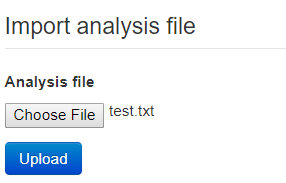
\includegraphics[scale=0.3]{pics/import.png}
    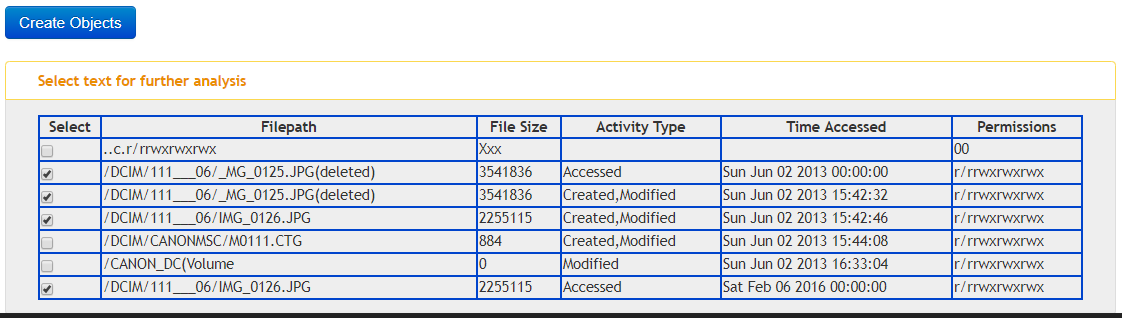
\includegraphics[scale=0.3]{pics/import-table.png}
    
    \begin{itemize}
        \item Possibility to import \textbf{Mactime} files [done]
        \item Pick only relevant files [done]
        \item \texttt{MISPObject} will be created [done]
    \end{itemize}
\end{frame}

\begin{frame}
        \frametitle{Data visualization (MISP 2.4.100/101?)}
    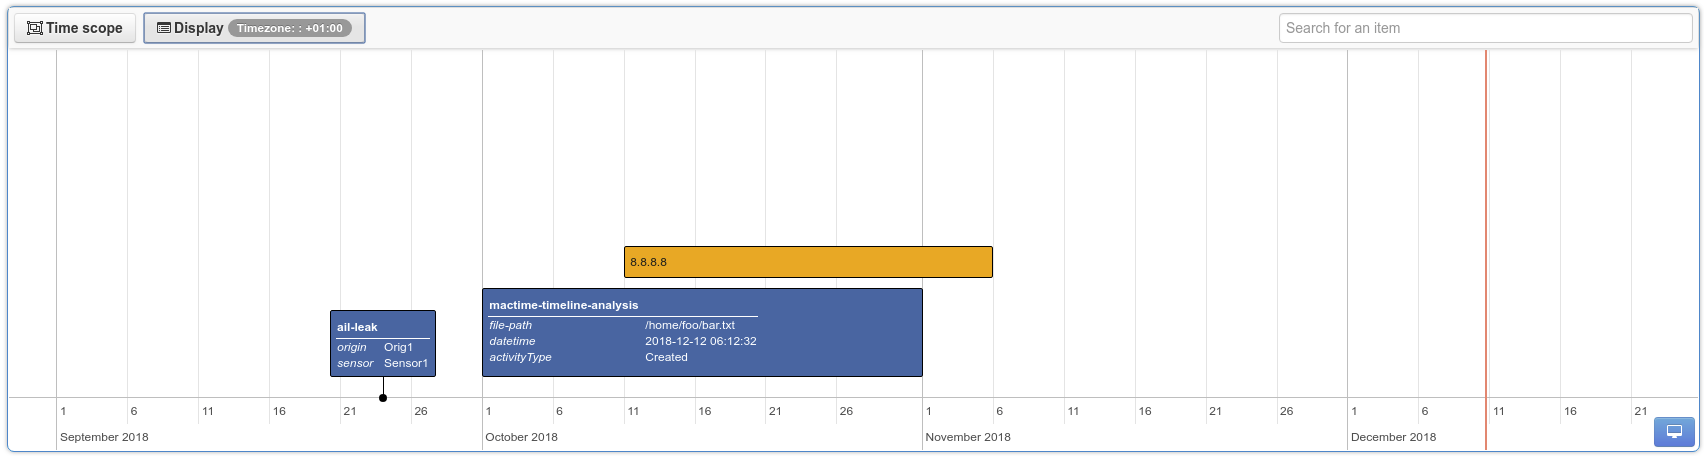
\includegraphics[width=1.0\linewidth]{pics/timeline.png}
    \begin{itemize}
        \item View: start-date only, spanning and search [dev-branch]
        \item Manipulate: Edit, Drag and Expand [dev-branch]
        \item Others: Timezone support [dev-branch]
    \end{itemize}

    \vspace{0.3cm}
    $\rightarrow$ For now [dev-branch], supports up to \textbf{micro-seconds} in the database and up to \textbf{milliseconds} in the web interface.
\end{frame}

\end{document}

